\section{Methods}
\label{sec:methods}

In this section, we present our matrix-matrix multiplix. Then explain our modifications to the triple matrix multiplications that are part of the AMG setup process.

\subsection{Matrix-Matrix Multiplication}
\label{sec:matmult}

%\subsubsection{Computation}
%\label{sec:comp}
Here we assume that the data is available locally, so we discuss it as a serial implementation. We have implemented \mm~ in a recursive fashion. We split the matrices recursively in two ways: split by half based on the matrix size, split by half based on number of nonzeros. First we explain the algorithms performing splitting based on the matrix sizes.

The recursive function, \recmm, includes three cases:
\begin{enumerate}
 \item Case 1: Stop the recursion: perform the multiplication.
 \item Case 2: A is horizontal.
 \item Case 3: A is vertical.
\end{enumerate}

\subsubsection{Case 1}
\label{sec:case1}
At the start of the recursive function, the number of nonzero rows of A ($A\_nnz\_row$) and nonzero columns of B ($B\_nnz\_col$) are being computed. A threshold for $\nnzsz = A\_nnz\_row \times B\_nnz\_col$ is set (for our experiments we use $20M$ \mr{explain why.}).
We continue splitting the matrices until the threshold is reached. Then, we preform the multiplication. We have implemented two methods for this case: dense data struture and hashmap.

%First method uses a dense matrix.
%The matrices are ordered as column-major.
In the first method, a dense matrix of size $\nnzsz$ is initialized to $0$. \mr{explain better:}Each nonzero of $B$ is multiplied by its corresponding nonzero of $A$ and the result will be added to the corresponding index in the dense matrix. At the end, we go through the dense matrix and add the nonzeros to the final multiplication matrix.

When $\nnzsz$ gets larger, it becomes inefficient to traverse the whole dense matrix and check for nonzeros in the final stage. To solve this issue, we have implemented another method that uses hashmaps. The entry's index is the key and its value is the hashmap's value. When we want to add the multipliation of nonzeros of $A$ and $B$ to the hashmap, we check if the index exists in the map. If it exists the value is being added to the existing one's. Otherwise a new entry will be added to the hashmap.

In Figure~\ref{fig:lap60}, we compare the two methods for a 3D Poisson problem of size $216k$. For $0 \leq \nnzsz \leq 10M$, in $1M$ steps, we show how which method is faster than the other one. For the lower range the first method is better and for the higher range the second one.

\begin{figure}[tbh]
 \centering
 \Description{Description}
 \includegraphics[width=8.5cm,height=4cm]{./figures/lap60_range.pdf}
 \caption{1}
 \label{fig:lap60}
\end{figure}

Figure~\ref{fig:eco} shows the same experiment for matrix ID $1882$ from SuiteSparse (Florida) Matrix Collection.

\begin{figure}[tbh]
 \centering
 \Description{Description}
 \includegraphics[width=8.5cm,height=4cm]{./figures/eco_range.pdf}
 \caption{1}
 \label{fig:eco}
\end{figure}

A combination of these two methods would give us the best of both. The dense method is being used for the lower range and the hashmap for the higher range. Figure ~\ref{fig:mix} compares the mixed method with the basic two methods.

\begin{figure}[tbh]
 \centering
 \Description{Description}
 \includegraphics[width=8.5cm,height=5cm]{./figures/mix.pdf}
 \caption{1}
 \label{fig:mix}
\end{figure}


\subsubsection{Case 2}
\label{sec:case2}
When A is horizontal, i.e. its row size is less than or equal to its column size, we halve A by column based on its cloumn size (Figure ~\ref{fig:case2}). Since row size of B eqauls column size of A, we halve B by row, so it will be a smiliar split to A, but horizontally. 

\begin{figure}[tbh]
 \centering
 \Description{Description}
 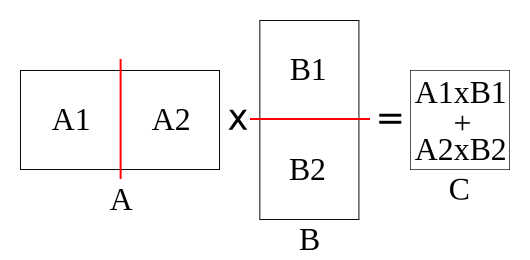
\includegraphics[width=6cm,height=2.7cm]{./figures/case2_001.pdf}
 \caption{}
 \label{fig:case2}
\end{figure}

\begin{algorithm}[H] 
  %\footnotesize
  \caption{Case 2: $C = \recmm2(A, B)$} \label{alg:case2} 
  \begin{algorithmic}[1]
    \Require $A$, $B$
    \Ensure  $C$
    \State $(A1, A2) = \spc(A)$
    \State $(B1, B2) = \spr(B)$
    \State $C1 \leftarrow \recmm(A1,B1)$
    \State $C2 \leftarrow \recmm(A2,B2)$
    %\State $C \leftarrow \textsc{mergesort}(C1, C2)$
  \end{algorithmic}
\end{algorithm}

\subsubsection{Case 3}
\label{sec:case3}
When A is vertical, i.e. its row size is greater than its column size, we halve A by row based on its row size and halve B by column (Figure ~\ref{fig:case3}). In contrary to the previous case, column size of B is not related to row size of A, so they are splitted independently.

\begin{figure}[tbh]
 \centering
 \Description{Description}
 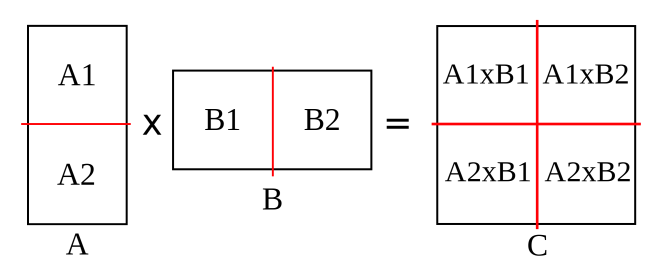
\includegraphics[width=6cm,height=2.5cm]{./figures/case3_001.pdf}
 \caption{1}
 \label{fig:case3}
\end{figure}

\begin{algorithm}[H] 
  %\footnotesize
  \caption{Case 3: $C = \recmm3(A, B)$} \label{alg:case3} 
  \begin{algorithmic}[1]
    \Require $A$, $B$
    \Ensure  $C$
    \State $(A1, A2) = \spr(A)$
    \State $(B1, B2) = \spc(B)$
    \State $C \leftarrow \recmm(A1,B1)$
    \State $C \leftarrow \recmm(A2,B1)$
    \State $C \leftarrow \recmm(A1,B2)$
    \State $C \leftarrow \recmm(A2,B2)$
    %\State $\textsc{sort}(C)$
  \end{algorithmic}
\end{algorithm}

\mr:{Explain the second method, splitting based on the number of nonzeros.}


\subsection{AMG Matrix Multiplication}
\label{sec:amg}

Short summary of AMG setup. Explain given the fine matrix, how coarsening is normally done, and where the triple matmult shows up as part of the Galerkin approximation. What else is done during setup. Basically, highlight that the matmult is the dominant part, and the part that is complex in parallel. 

% original text starts here 
To compute the coarse matrix $Ac$, a triple matrix multiplication should be done:
\begin{equation}
 Ac = R \times A \times P
\end{equation}
in which $R = P^T$.

This section includes two parts: First, we describe preforming the multiplication locallly on one processor. In the next part, we explain how the communication of the matrix data is being done between processors.

%\subsubsection{Communication}
%\label{sec:comm}

Matrices are partitioned on multiple processors by row blocks (Figure~\ref{fig:partition}). Matrices $A$ and $P$ have the same number of rows and consequently are partitioned the same way. $R$ has less number of rows and has a different partition.

\begin{figure}[tbh]
 \centering
 \Description{Description}
 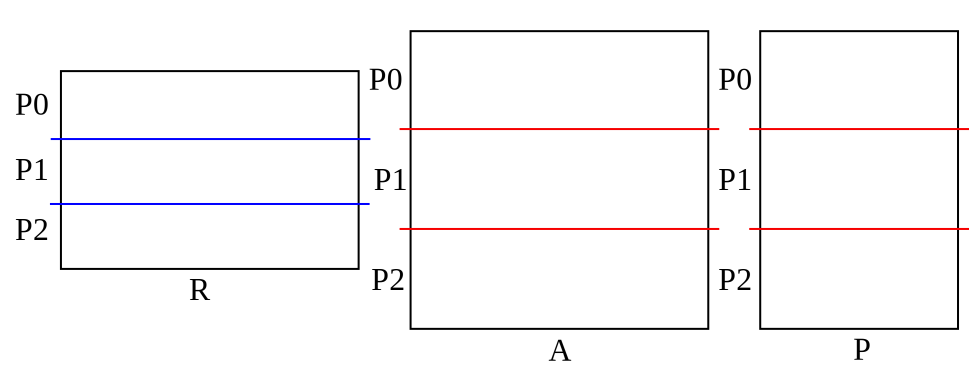
\includegraphics[width=8cm,height=3cm]{./figures/partition.pdf}
 \caption{1}
 \label{fig:partition}
\end{figure}

The triple matrix product is being done in two parts: first $A \times P$, then $R \times B$, in which $B = A \times P$, so performing matrix-matrix multiplications (\mm) twice.

\subsubsection{Part 1}

In this part, we compute $B := A \times P$. We assume the same partition of rows of $A$ on its columns. The same partition of rows of $R$ is assumed on columns of $P$ (Figure~\ref{fig:part1b}).
Here we consider doing \mm ~on processor $P1$. To compute entry $B(i, j)$, we need to multiply row $i$ of $A$ with column $j$ of $P$ and add them together (since we are working with sparse matrices, we only consider the nonzeros).

\begin{figure}[tbh]
 \centering
 \Description{Description}
 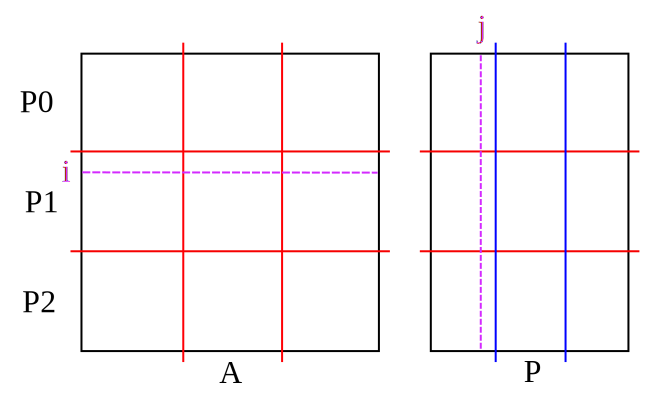
\includegraphics[width=5.5cm,height=3cm]{./figures/part1b.pdf}
 \caption{1}
 \label{fig:part1b}
\end{figure}

Column $j$ is distributed between all the processors, so we will be able to perform  summation $B_{ij} = \sum_{k} A_{ik} P_{kj}$, after communicating all nonzeros of column $j$ and performing the multiplication. (explain this part clearer and show why this method is not good). To avoid that, we can use the fact that $R$ is the transpose of $P$ and we already have computed it. We note that column blocks of $P$ (e.g. $r0$ in Figure~\ref{fig:part1c}) are actually row blocks of $R$ transposed ($rt0$, which is transpose of $r0$).

\begin{figure}[tbh]
 \centering
 \Description{Description}
 \includegraphics[width=5.5cm,height=3cm]{./figures/part1c.pdf}
 \caption{1}
 \label{fig:part1c}
\end{figure}

Algorithm \ref{alg:part1} shows how we do it in an overlapped fashion using MPI. $B_{i}$ is the row block of matrix $B$ on processor $i$ and $B_{ik}$ is the sub-block result of multiplying $A_i$ with $rt_i$.

\begin{algorithm}[H] 
  %\footnotesize
  \caption{Part 1: $B_i = A_i \times P$} \label{alg:part1} 
  \begin{algorithmic}[1]
    \Require $A_i$, $R$
    \Ensure  $B_i$ (result of $A_i \times P$)
    \State $R1 \leftarrow$ transpose of $R_i$ (locally)
    \For{$k=myrank:myrank+nprocs$}
      \State $R2 \leftarrow\ Irecv(transpose\ of\ R)\ from\ right\ neighbor$
      \State $Isend(R1)\ to\ left\ neighbor$
      \State $B_{ik} \leftarrow \recmm(A_i, R1)$ 
      \State $wait\ for\ Isend\ and\ Irecv\ to\ finish$
      \State $swap(R1,R2)$
    \EndFor
    \State locally sort $B_i$ and add duplicates
  \end{algorithmic}
\end{algorithm}


\subsubsection{Part 2}

Now we explain how to do the second \mm: $R \times B$, in which $B = A \times P$. Figure~\ref{fig:part2d} shows an example on processor $P1$. The blocks of $R$ on processor $P1$ should be multiplied with the corresponding blocks of $B$ with the same color. To do that we need to communicate whole $B$ between all the processors.

\begin{figure}[tbh]
 \centering
 \Description{Description}
 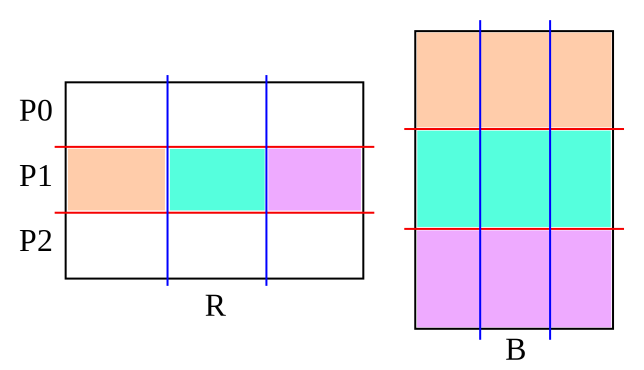
\includegraphics[width=5.5cm,height=3cm]{./figures/part2d.pdf}
 \caption{1}
 \label{fig:part2d}
\end{figure}

To avoid this expensive communication, we again can use the fact that we already have computed the transpose of $R$. We only perform the multplication of the green blocks on processor $P1$ in Figure~\ref{fig:part2e}, which can be done locally.

\begin{figure}[tbh]
 \centering
 \Description{Description}
 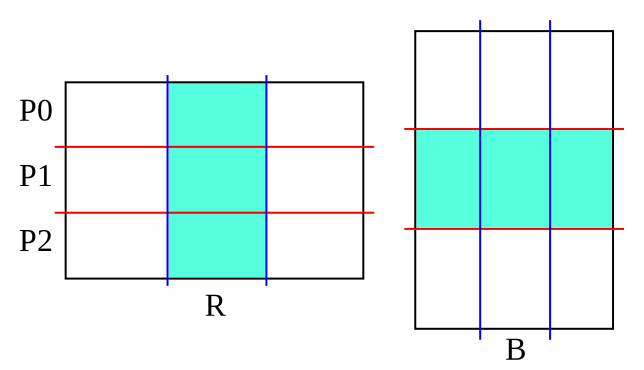
\includegraphics[width=5.5cm,height=3cm]{./figures/part2e.pdf}
 \caption{1}
 \label{fig:part2e}
\end{figure}

Using this method, we need to add duplicates twice (explain duplicates). Once, after doing the multplication; Second time, after sorting the result globally and putting the entries on the correct processors. Algorithm~\ref{alg:part2} shows how we have implemented it. Note that each sub-block of $R_i$ should be multiplied by whole $B_i$, in contrary to the naive method, in which each sub-block of $R_i$ is multiplied by only one other sub-block of $B_i$.

\begin{algorithm}[H] 
  %\footnotesize
  \caption{Part 2: $Ac = R \times B$} \label{alg:part2} 
  \begin{algorithmic}[1]
    \Require $P_i$, $B_i$
    \Ensure  $Ac_i$
    \State $PT_i \leftarrow$ transpose of $P_i$ (locally)
    \For{$k=0:nprocs$}
      \State $Ac_i \leftarrow \recmm(PT_{ik}, B_i)$
    \EndFor
    \State locally sort $Ac_i$ and add duplicates
    \State globallly sort $Ac_i$ and add duplicates
  \end{algorithmic}
\end{algorithm}
